Una tienda de helados vende 2 bolas de helado por \$5 dólares. Cada bola adicional cuesta \$1 dolar.

\begin{multicols}{2}
    \begin{parts}
        \part Completa la Tabla \ref{tab:bolas_helado} para representar la relación.

        \renewcommand{\arraystretch}{1}
        \begin{table}[H]
            \rowcolors{2}{colorrds!10}{lightgray!10}
            \centering
            \caption{Costo de un helado según la cantidad de bolas.}
            \label{tab:bolas_helado}
            \begin{tabular}{|c|c|c|}
                \toprule
                \rowcolor{colorrds!80}
                \textbf{\color{white}Bolas de helado} & \textbf{\color{white}Costo} & \textbf{\color{white}Coordenada}                 \\\midrule
                2                                     & \$5                         & \ifprintanswers$( 2 ,5)$\else( \quad,\quad )\fi  \\\hline
                3                                     & \ifprintanswers \$6 \fi     & \ifprintanswers$( 3 ,6)$\else( \quad,\quad )\fi  \\\hline
                4                                     & \ifprintanswers \$7 \fi     & \ifprintanswers$( 4 ,7)$\else( \quad,\quad )\fi  \\\hline
                5                                     & \ifprintanswers \$8 \fi     & \ifprintanswers$( 5 ,8)$\else( \quad,\quad )\fi  \\\hline
                6                                     & \ifprintanswers \$9 \fi     & \ifprintanswers$( 6 ,9)$\else( \quad,\quad )\fi  \\\hline
                7                                     & \ifprintanswers \$7 \fi     & \ifprintanswers$( 7 ,10)$\else( \quad,\quad )\fi \\\hline
                8                                     & \ifprintanswers \$8 \fi     & \ifprintanswers$( 8 ,11)$\else( \quad,\quad )\fi \\\hline
                9                                     & \ifprintanswers \$9 \fi     & \ifprintanswers$( 9 ,12)$\else( \quad,\quad )\fi \\\hline
                \bottomrule
            \end{tabular}
        \end{table}

        \columnbreak

        \part Con ayuda de los pares ordenados de la Tabla \ref{tab:bolas_helado}, grafica los datos en el plano cartesiano.

        \begin{figure}[H]
            \centering
            \ifprintanswers
                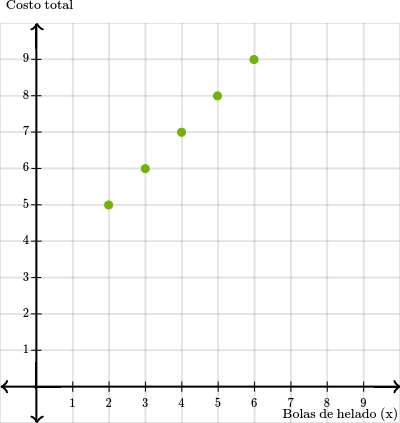
\includegraphics[width=0.6\linewidth]{../images/20230321002620}
            \else
                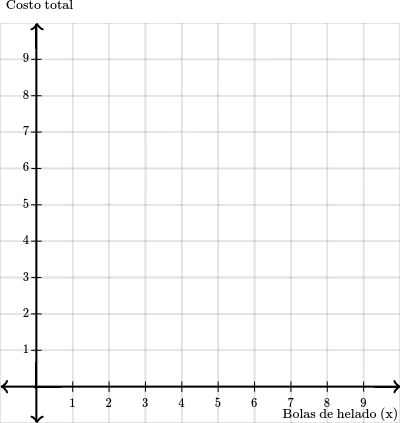
\includegraphics[width=0.6\linewidth]{../images/20230321002620_blank}
            \fi
        \end{figure}
    \end{parts}%
\end{multicols}%
